This section of the report includes excerpts from research publications produced by groups using the open data lab. We highlight a couple MSDS capstone projects (\ref{sec:BMC} and \ref{sec:wik}) as well as a faculty research project (\ref{sec:hmt}) and the undergraduate machine learning club (\ref{sec:mlc}).

\section{Bourne/Mura Capstone}
\label{sec:BMC}

\emph{Sean Mullane, Ruoyan Chen, Sri Vaishnavi Vemulapalli, Eli J. Draizen, Ke Wang, Cameron Mura, asnd Philip E. Bourne}
\bigskip

The biological function of a protein stems from its 3D structure. Understanding these functions is important in biomedical research. Given the high costs of using experimental means to determine protein structures, current methods do not scale. As a result, many have attempted to apply machine learning to this problem to predict structure from amino acid sequence data.

Our work focuses on a sub-problem of this field: predicting locations of the capping motifs which terminate $\alpha$-helix protein structures. These motifs have only been described empirically to date~\cite{ref:bmc}. As a step toward a robust and statistically-based understanding of helix capping, we demonstrate that machine learning modules can be trained to predict helix cap positions from sequence data.

\begin{figure}[!hbtp]
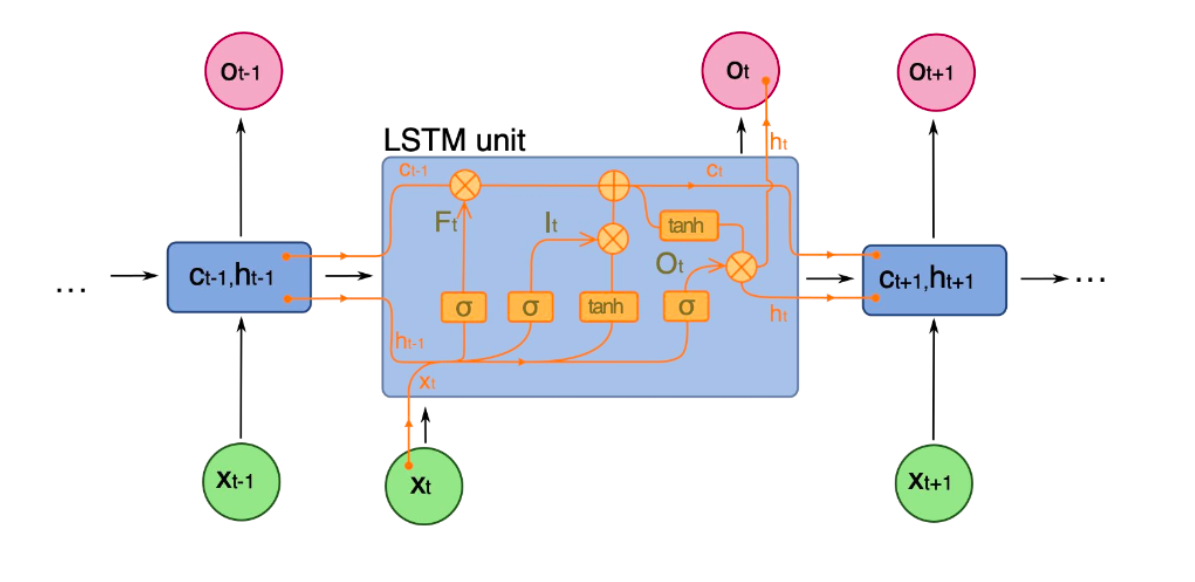
\includegraphics[width=\textwidth]{images/bmc1}
\caption{LSTM with feature vectyor of single amino acid residue as input to each cell}
\end{figure}

\begin{figure}[!hbtp]
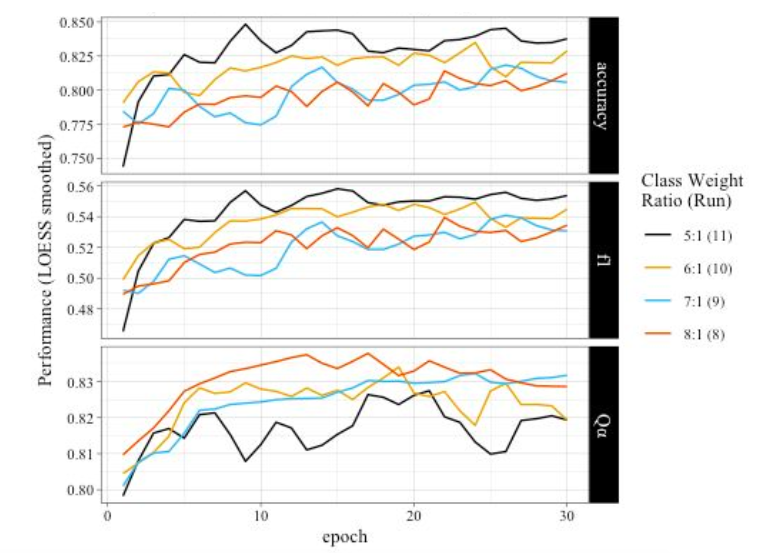
\includegraphics[width=\textwidth]{images/bmc2}
\caption{Effect of Loss Function Weighting}
\end{figure}



From poster presented at SIEDS 2019.

\section{DSI Wiki}
\label{sec:wik}

\emph{Charu Rawat, Arnab Sarkar, Sameer Singh, Rafael Alvarado, and Lane Rasberry}
\bigskip

In this paper, we propose a framework to understand and detect abuse in the English Wikipedia community. We analyze multiple publicly available data sources provided by Wikipedia. We propose a web scraping methodology to extract user-level data and perform extensive exploratory data analysis to understand the characteristics of users who have been blocked for abusive behavior in the past.

We further build upon these insights to develop an abuse detection model that leverages Natural Language Processing techniques, such as character and word n-grams, sentiment analysis, and topic modeling, to generate features that are used as inputs in a model based on machine learning algorithms to predict abusive behavior.

\begin{figure}[!hbtp]
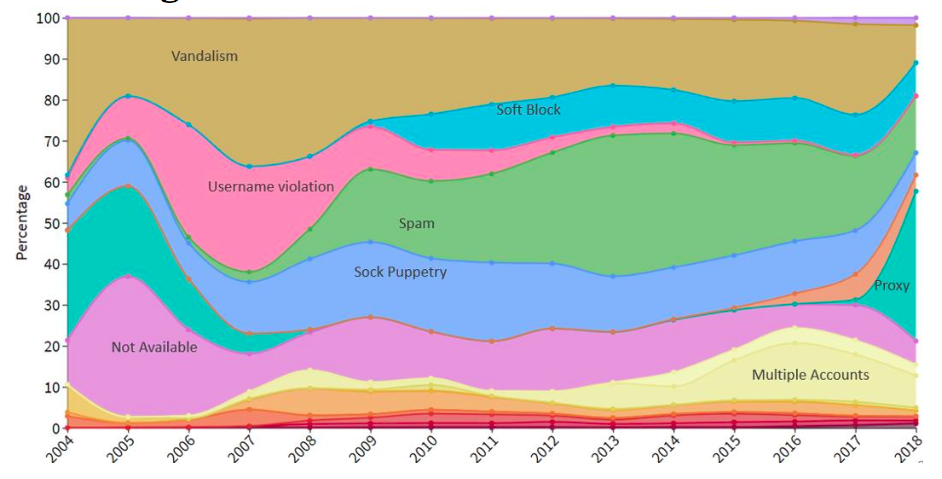
\includegraphics[width=\textwidth]{images/wiki1}
\caption{Share of block reasons over time}
\end{figure}

\begin{figure}[!hbtp]
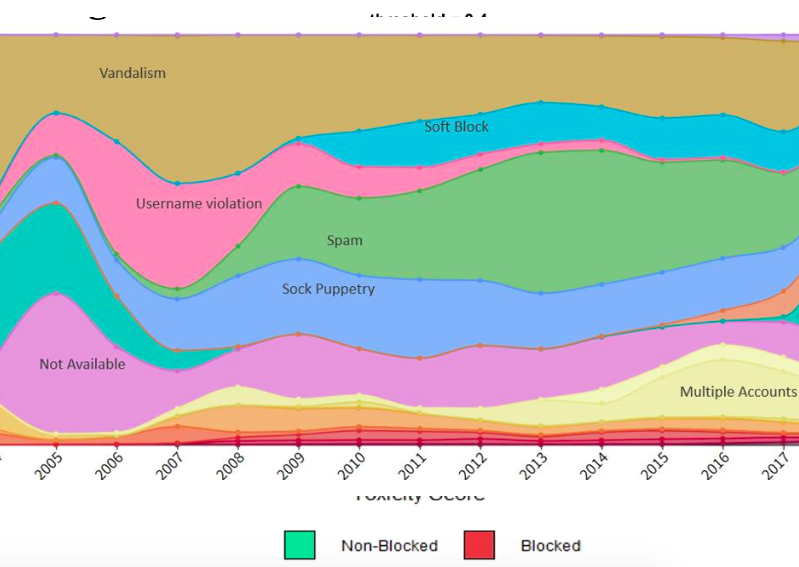
\includegraphics[width=\textwidth]{images/wiki2}
\caption{Toxicity score evaluation}
\end{figure}

From poster presented at SIEDS 2019.

\section{Healthy Markets}
\label{sec:hmt}

\section{Undergraduate Machine Learning Club}
\label{sec:mlc}
This semester, the Undergrad ML group built the foundations of a new Deep Reinforcement Learning platform. At its center is an implementation of Proximal Policy Optimization with Random Network Distillation. This technique, first published by OpenAI in late 2018, augments the PPO learning algorithm with the 'curiosity' to find novel states - greatly increasing performance in environments with sparse rewards by giving the agent continuous intrinsic ones. Our version is currently geared towards vision-based video game tasks; so far it supports any pixels-only environment from both Gym and Gym-Retro, but can be modified to work with any similar RL package. While the original paper came with an open source implementation, our version is more general purpose and written in TensorFlow's eager execution mode, which will make it easier to extend, debug and maintain going forward. It is also very scalable: we use synchronous gradient descent to process small amounts of data (a single rollout) on each worker, which eliminates the need for a GPU and lets us take full advantage of CPU clusters.

So far we have primarily tested the agent on Sonic The Hedgehog. While not as difficult an exploration environment as famous benchmarks like Montezuma's Revenge, Sonic is an interesting problem because of its very inconsistent difficulty. Long stretches of running right and jumping are broken up by obstacles that require significant long-term planning, creating bottlenecks that tend to destabilize training and require the agent to try new strategies over and over again. Our agent performs surprisingly well, even with just a few parallel workers. Here is an example chart of the training process, which shows the map and the agent's deaths, as well as the internal and external rewards.

\begin{figure}[!hbtp]
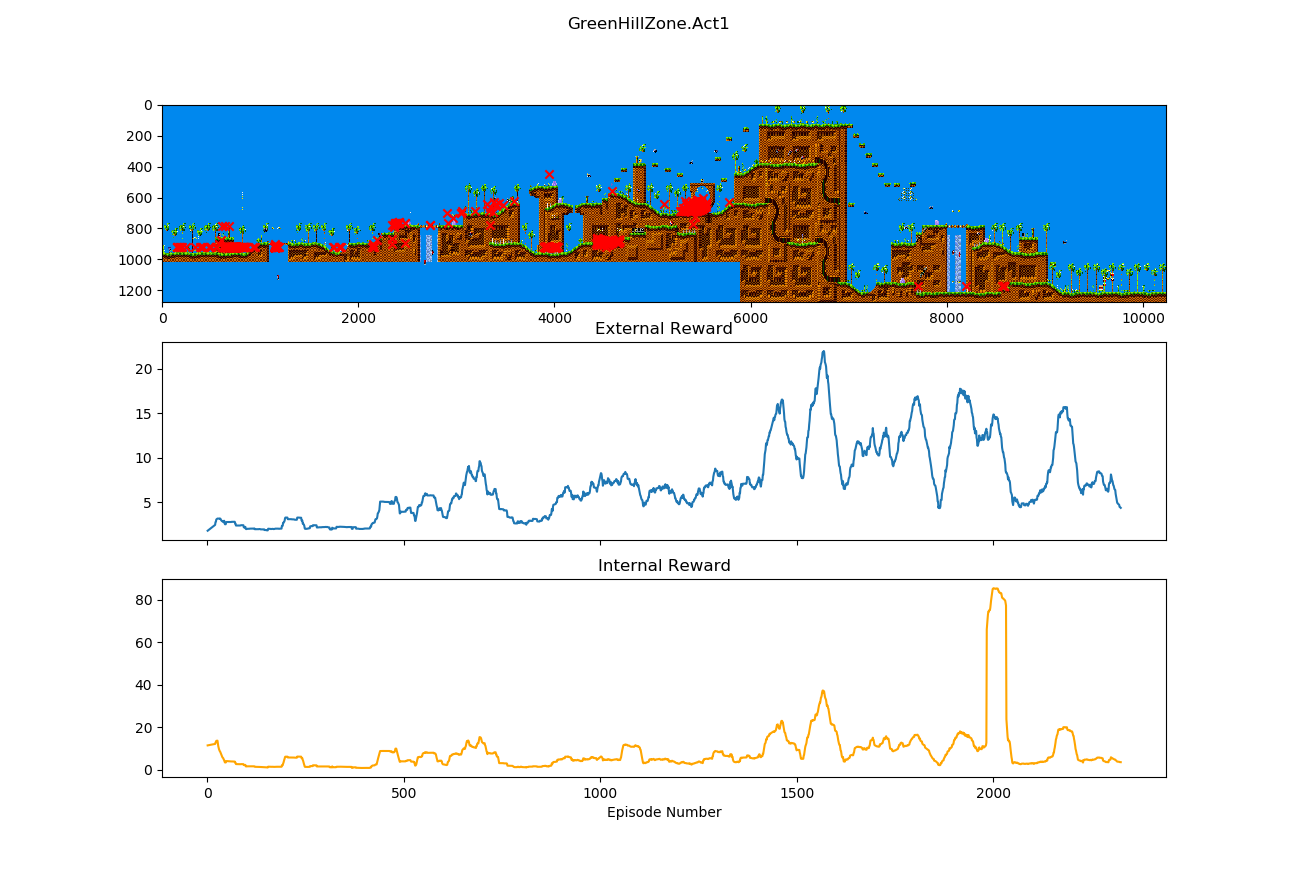
\includegraphics[width=\textwidth]{images/mlunder_figure}
\caption{Example chart of the training process, which shows the map and the agent's deaths, as well as the internal and external rewards. \cite{github:mlunder} }
\end{figure}


%Proximal Policy Optimization with Random Network Distillation  -- https://arxiv.org/abs/1810.12894



